%% 
%% 
%% 

\chapter{Related Work and Background}
\label{cha:RelatedWorks}

\section{MRFs and Energy Function}
\subsection{Markov Random Fields}
\label{sec:MRF}
\emph{Markov Random Fields} are also known as \emph{undirected
  graphical model} can be seen as a regularized joint
log-probability distribution of arbitrary non-negative functions
over a set of maximal cliques of the
graph~\cite{bishop:2006:PRML}. Let $C$ denotes a maximal clique
in one graph and $\by_C$ denotes the set of variables in that
clique. Then the joint distribution can be written as:
\begin{align}
  p(\by)=\frac{1}{Z}\prod_{C}{\Psi_C(\by_C)}
\end{align}
\noindent where $\Psi$ is called \emph{potential functions} which
can be defined as any non-negative functions and
$Z=\sum_{\by}\prod_{C}{\Psi_C(\by_C)}$ which is a normalization
constant. To infer labels which best explains input data set, we
can find the \emph{maximum a posteriori} (MAP) labels by solving
$\by^*=\argmax_{\by}p(\by)$. Because potential functions are
restricted to be non-negative, it gives us more flexible
representations by taking exponential of those terms. Thus the
joint distribution becomes:
\begin{align}
  p(\by)=\frac{1}{Z}exp(-\sum_{C}{E_C(\by_C)})
\end{align}
\noindent where $E$ is called \emph{energy functions} which can be
arbitrary functions. Therefore, \emph{maximum a posteriori}
problem is equivalent to \emph{energy minimization} problem,
which is also known as \emph{inference}:
\begin{align}
  \by^*=\argmax_{\by}p(\by)=\argmin_{\by}(-\sum_{C}{E_C(\by_C)})
\end{align}
To optimize the performance we can also consider a weighted
version of energy functions. In order to do this we can decompose
energy functions over nodes $\N$, edges $\E$ and higher order
cliques $\C$~\cite{Szummer:ECCV08} then add weights on them
accordingly. Let $\bw$ be the vector of parameters and $\phi$ be
arbitrary feature function, then the energy can be decomposed as
a set linear combinations of weights and feature vectors:

\begin{align}
  \label{eq:energyfunction_UPH}
  E(\by;\bw)=\sum_{i\in \N}{\bw_i^U\phi^U(\by_i)}+
  \sum_{(i,j)\in \E}{\bw_{ij}^P\phi^P(\by_i,\by_j)}+
  \sum_{\by_C\in \C}{\bw_C^H\phi^H(\by_C)}
\end{align}

\noindent where $U$ denotes \emph{unary} terms, $P$ denotes
\emph{pairwise} terms and $H$ denotes \emph{higher order} terms
(when $|C|>2$ namely each clique contains more than two
variables).

A weight vector $\bw$ is more preferable if it gives the
ground-truth assignments $\by_t$ less than or equal to energy
value than any other assignments $y$:

\begin{align}
E(y_t,w)\leq E(y,w)~ \text{,~}\forall y \neq y_t
\text{,~} y\in \Y
\end{align}


Thus the goal of \emph{learning} MRFs is to learn the parameter
vector $\bw^*$ which returns the lowest energy value for the
ground-truth labels $y_t$ relative to any other assignments
$y$~\cite{Szummer:ECCV08}:

\begin{align}
\bw^* = argmax_{\bw}(E(y_t,w)-E(y,w))~ \text{,~}\forall y \neq y_t
\text{,~} y\in \Y
\end{align}

So far we have introduced three main research topics of MRFs:
definition of \emph{energy function} (potential functions),
\emph{inference} problem (MAP or energy minimization) and
\emph{learning} problem.

As for energy function, our work focus on a generalization of
k-means clustering known as Gaussian Mixture Models to
incorporate information about the covariance structure of the
data as well as the centers of the latent Gaussians. The
grabcut~\cite{Rother:SIGGRAPH04} algorithm is used to train GMMs
and the final results are used to construct the unary terms. For
pairwise terms, we use the Potts model introduced by
\citename{Kohli:CVPR07} to encode pairwise consistency. The
\emph{inference} problem is solved by using a
graph-cut~\cite{Boykov:ICCV99, Boykov:PAMI04} algorithm and the
max margin framework~\cite{tsochantaridis2005large} has been
addressed to learn parameters of the energy function.

\subsection{Construction of stocks relationship graph}
\label{sec:con_stock_graph}

The stock market is a complicated system with many variables
affecting whether or not a particular stock price goes up or
down. In order to accurately capture the complex relationships
between companies that affect their stock prices, they can be
represented as an undirected graph (MRFs). Each node in the graph
corresponds to a single company and each edge represents
collaboration between a pair of companies. This work uses the
companies appearing in the information technology sector of the
\emph{ HS300 } index. Because the relationship of collaborating
companies is many-to-many, this would normally be an intractable
problem if inference were determined using a message-passing
algorithm (the complexity is exponential in the tree-width of the
graph). Fortunately, the collaboration relationship is an
associative one (i.e. if two companies are collaborators, an
increase in the stock price of one of them is likely associated
with an increase for the other; likewise, a decrease in the stock
price of one of them is likely associated with a decrease for the
other). As mentioned earlier, we are able to use minimum cuts to
solve inference queries in polynomial time. Edges in the graph
are determined by comparing the estimated result count in the
\emph{ Sougo } search engine for the two queries:

1.  “Company A”-“Company B” collaboration

2.  “Company A”-“Company B” competition

If the first query has more than 1.5 times the results of the
second, an edge is added to the graph connecting the nodes for
Company A and Company B. This multiplier is necessary to avoid
adding edges between companies that are either not strong
collaborators or competitors and thus have extremely similar
result counts for both queries. Our spider code together with
graph data are available on Github
\url{https://github.com/spacegoing/sogou_spider}. The unary terms are
measured using GMMs and pairwise terms are measured using Potts
model, requiring the SSVM to learn the labelling from the feature
vectors at the nodes.

\subsection{Configuration of Energy Function}
\label{sec:grabcut}

\begin{figure}[b]
  \centering
  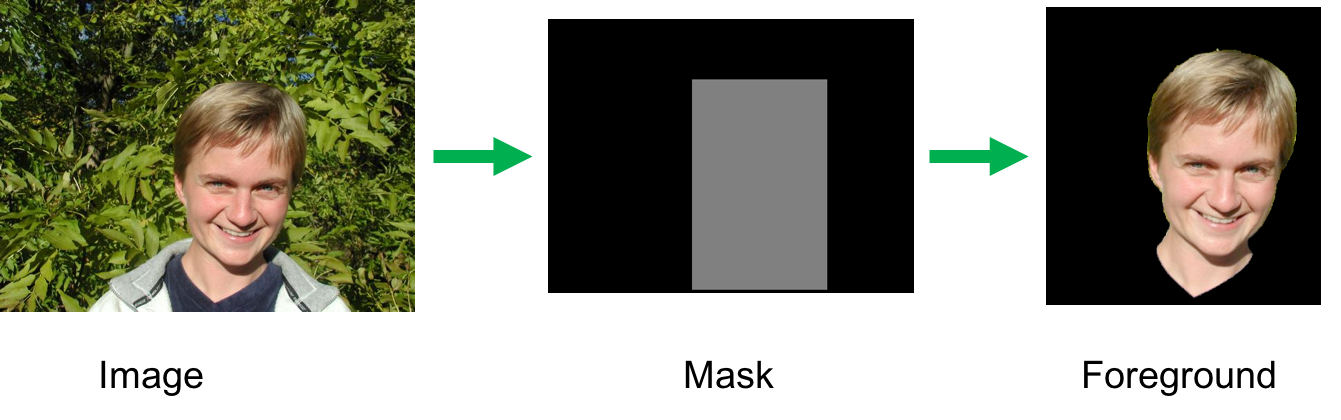
\includegraphics[width=1\linewidth]{RelatedWorks/figures/grabcut_task.png}
  \caption{\label{fig:grabcut_example} Picture on the left is
    the original picture. Picture
    on the middle is a user defined mask. The task is to extract
    foreground pixels within that rectangle. On the right is the
    ground truth foreground.}
\end{figure}

In this section we described the configuration of our energy
function. We mainly introduce the \emph{GrabCut} algorithm which
we used to generate our unary terms. The \emph{Potts model} is
used as our pairwise terms. Thus our energy function can be
written as:
\begin{align}
  \label{eq:energyfunction_UP}
  E(\by;\bw)=\theta^U\sum_{i\in \N}{\bw_i^U\phi^U(\by_i)}+
  \theta^P\sum_{(i,j)\in \E}{\bw_{ij}^P\phi^P(\by_i,\by_j)}
\end{align}
\noindent where $\theta^U$ and $\theta^P$ are parameters to be
optimized.

The \emph{GrabCut} algorithm was proposed
by~\citename{Rother:SIGGRAPH04} in order to solve background
foreground segmentation problem (see
figure~\ref{fig:grabcut_example}). They first defined MRFs over
an labeled image and then use
\emph{graph-cuts}~\cite{Boykov:ICCV01} method to do the
inference. In this section we use two of their contributions:
estimating color distribution (foreground and background) using
\emph{Gaussian Mixture Models} (GMMs) and an \emph{EM} like
two-step algorithm to train their model.

Suppose there are $N$ pixels in an image. In order to construct
MRFs, they first defined an energy
function~\eqref{eq:energyfunction_UPH} with unary and pairwise
terms:

\begin{align}
  \label{eq:grabcut_energy}
  G(\alpha, \bk, \btheta, \bz) = 
  \sum_{i\in \N}{\psi^U(\alpha_i, \bk_i, \btheta, \bz_i)}+
  \sum_{(i,j)\in \E}{\psi^P(\alpha_i,\bz_i)}
\end{align}
where $i$ is the index of pixels, $\alpha \in {0,1}$ is the label
for pixel $i$. $0$ is for the background and $1$ is for the
foreground. $\bz$ denotes the pixel vector in RGB color space.
$\bk$ and $\btheta$ are all parameters vectors and will be
explained in the next paragraph. 

\begin{algorithm}[tb]
  \begin{algorithmic}[1]
    \REPEAT
    \STATE{\emph{Assign GMM components} to stocks: \\
      $\bk_i^*=\argmin_{\bk_i}\psi^U(\alpha_i, \bk_i, \btheta,
      \bz_i)$}
    \STATE{\emph{Learn GMM parameters} from data z:\\
      $\btheta=\argmin_{\btheta}\sum_{i\in \N}{\psi^U(\alpha_i, \bk_i, \btheta, \bz_i)}$}
    \STATE{\emph{Estimate segmentation}: graph-cuts inference:\\
      $\min_{\alpha}\min_{\bk}E(\alpha, \bk, \btheta, \bz)$}
    \UNTIL{convergence}
  \end{algorithmic}
  \caption{\label{alg:grabcut} GrabCut training algorithm}
\end{algorithm}

In our configuration, we use the graph described
in~\ref{sec:con_stock_graph} in replacement of the image. Each
node in the graph represents a stock instead of pixel and the
edge between stocks represents their pairwise relationship. The
label $\alpha \in {0,1}$ equals $1$ when the stock price has a
positive movement, and vice versa. $\bz$ denotes the stock's
market price vector instead of pixel's RGB value. Other
parameters are the same with their configurations.

The \emph{Gaussian Mixture Models} (GMMs) with $K$ components
(typically $K=5$) is used for generating unary terms. Two GMMs,
one for positive movement and one for negative movement, are
jointly trained by the algorithm.
$\bk={\bk_1,\dots,\bk_i,\dots,\bk_N}$ with $\bk_i\in 1,\dots,K$
assigns each stock (node) $i$ to a unique GMMs component. The
component is either belonging to positive movement's GMMs or
negative movement's GMMs, which is depended on the label
$\alpha_i\in {0,1}$. $\btheta$ is the parameter vector which
contains parameters of standard GMMs plus \emph{mixture weighting
  coefficients}~\cite{Rother:SIGGRAPH04}.

The pairwise function $\psi^P$ in \eqref{eq:grabcut_energy} is
defined as a smoothness indicator which measures both feature
vector (stock price vector) and spatial distances (graph
distances) simultaneously. It is used to encourage coherence of
similar pixel pairs. This energy function was later used to
construct an \emph{st min-cut} graph which can be inferred
efficiently using \emph{graph-cuts}~\cite{Boykov:ICCV01}
algorithm. This gives some insights to their second contribution.

To optimize the performance, a two-step learning algorithm is
used. The algorithm first re-assign GMMs components ($\bk$) to
each pixel then update parameters $\btheta$ with new assignments.
The result of the trained GMMs are used directly into
\emph{graph-cuts} algorithm~\ref{alg:grabcut} as unary terms.
Finally the label $\alpha_i$ for each pixel $i$ is inferred
jointly using \emph{graph-cuts} algorithm. This whole procedure
is repeated until convergence (or reaches termination
conditions). We briefly summarized this procedure in
\algref{alg:grabcut}

In this thesis we use GMMs trained by GrabCut algorithm for our
unary terms $\phi^U$ in equation~\eqref{eq:energyfunction_UP}.

The pairwise function $\phi^P$ in our energy
function~\eqref{eq:energyfunction_UP} is defined as a Potts
model:

\begin{align}
  \label{eq:energyfunction_pairwise}
  \phi^P(\by_i,\by_j)=
  \begin{cases}
    0 & \text{if} x_i = x_j \\
    \psi^P_{ij}(y_i, y_j) = \frac{\lambda}{d_{ij}} \ind{y_i \neq
      y_j} \exp\left\{- \frac{\|x_i - x_j\|^2}{2 \beta}\right\} &
    \text{otherwise}
  \end{cases}
\end{align}

\noindent where $d_{ij}$ is the graph distance between stocks $i$
and $j$. $x_i$ and $x_j$ are stock market price vectors.

\subsection{Exact Inference}
\label{sec:exact_inference}

Exact inference on MRFs has been extensively studied in past
years. Researchers found that, energy functions which can be
transformed into quadratic pseudo-Boolean
functions~\cite{Ishikawa:PAMI03,Ishikawa:CVPR09,Rother:CVPR09}
are able to be minimized exactly using \emph{graph-cuts} like
algorithms~\cite{Freedman:CVPR05,Hammer:1965} when they satisfy
submodularity condition~\cite{Boros:MATH02}.
\citename{Kohli:TR08} and \citename{Gould:ICML2011} adapted those
results to perform exact inference on lower linear envelope
potentials. In this section we mainly focus on describing the
\emph{st min cut} graph constructed for energy function containing
unary and pairwise potentials.

Following the approach of \citename{Kohli:CVPR10},
\citename{Gould:ICML2011,gouldlearning} transformed the MRFs into
a quadratic pseudo-Boolean function by introducing $K-1$
auxiliary variables $\bz = \left(z_1, \ldots, z_{K-1}\right)$
with $z_k\in \{0,1\}$:

\begin{align}
  E^c(\by_c, \bz) = a_1 W_{\!c}(\by_c) + b_1
  {}+ \sum_{k = 1}^{K-1} z_k \left( \left(a_{k+1} - a_k\right) W_{\!c}(\by_c) + b_{k+1} - b_k \right)
  \label{eqn:binary_concave_z}
\end{align}

\noindent for a single clique $c \in \C$. Under this formulation,
\citename{Gould:ICML2011,gouldlearning} showed that minimizing
the pseudo-Boolean function over $\bz$ is equivalent to selecting
(one of) the active functions(s) from equation. Another important
property of optimized $\bz$ under this formulation is that it
automatically satisfies the constraint~\cite{gouldlearning}:

\begin{figure}[t]
  \centering
  \setlength{\tabcolsep}{2pt}
  \begin{tabular}{cc}
    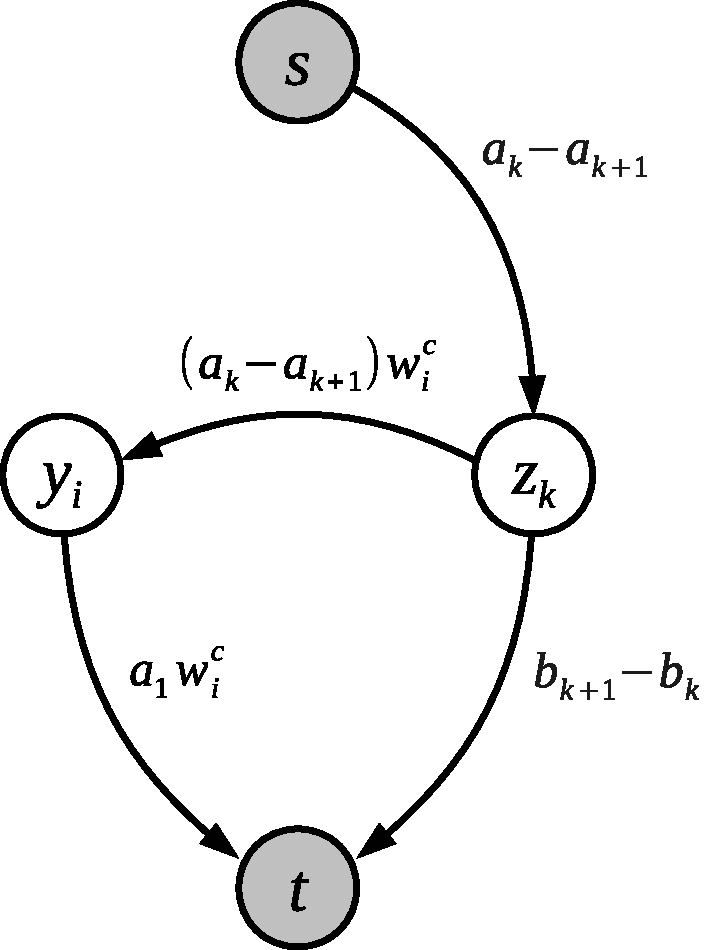
\includegraphics[width=0.45\columnwidth]{Methodology/figures/stmincut}&
                                                                         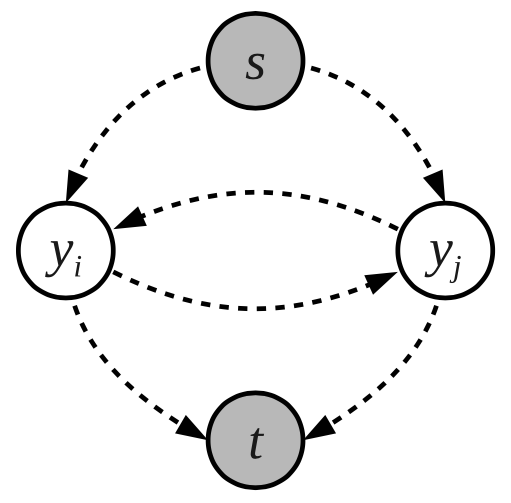
\includegraphics[width=0.5\columnwidth]{Methodology/figures/unary_pairwise.png}\\
                                                                         {\small (a)} & {\small (b)} 
  \end{tabular}
  \caption{\label{fig:stmincut} $st$-graph
    construction~\cite{gouldlearning} for
    equation~\eqref{eqn:posiform}, unary and pairwise terms.
    Every cut corresponds to an assignment to the random
    variables, where variables associated with nodes in the
    ${\cal S}$ set take the value one, and those associated with
    nodes in the $\T$ set take the value zero. With slight abuse
    of notation, we use the variables to denote nodes in our
    graph.}
\end{figure}

\begin{align}
  \label{eq:z_consecutive_constraint}
  z_{k+1} \leq z_k
\end{align}

In order to construct the \emph{st-min-cut} graph,
\citename{gouldlearning} rewrote
equation~\eqref{eqn:binary_concave_z} into
\emph{posiform}~\cite{Boros:MATH02}:

\begin{align}
  \label{eqn:posiform}  
  E^c(\by_c, \bz)
  &= b_1 - (a_1 - a_K) + \sum_{i \in c} a_1 w^c_i y_i
  {}+ \sum_{k = 1}^{K - 1} \left( b_{k+1} - b_k \right) z_k\\
  &+ \sum_{k = 1}^{K - 1} \left( a_k - a_{k+1} \right) \bar{z}_k
  {}+ \sum_{k = 1}^{K - 1} \sum_{i \in c} \left( a_k - a_{k+1}
    \right) w^c_i \bar{y}_i z_k \nonumber
\end{align}

\noindent where $\bar{z}_k = 1 - z_k$ and $\bar{y}_i = 1 - y_i$.
$a_1$ is assumed to be greater than $0$ so that all coefficients
are positive. After proving \emph{submodularity} of the energy
function~\eqref{eqn:posiform}, \citename{gouldlearning}
constructed the \emph{st-min-cut} graph based on
equation~\eqref{eqn:posiform}.

The construction is explained in \figref{fig:stmincut}. Figure
(a) denotes construction for equation~\eqref{eqn:posiform}.
Figure (b) denotes construction for unary and pairwise terms (see
\cite{Kolmogorov:PAMI04}). For unary edges (4 edges on both
sides), weights on each edge are corresponding to values in input
unary terms accordingly. For pairwise edges (2 edges in the
middle), both edges share the same weight which equals to the
input pairwise term.



% %%% Local Variables:
% %%% mode: latex
% %%% TeX-master: "../thesis"
% %%% End:

